\documentclass[11pt,a4paper]{article}

\usepackage[margin=1in]{geometry}
\usepackage{amsmath,amssymb}
\usepackage{booktabs}
\usepackage{graphicx}
\usepackage{array}
\usepackage{longtable}
\usepackage{float}
\usepackage[hidelinks]{hyperref}

\graphicspath{{../figures/}}

\title{Homework 1\\Network Dynamics and Learning}
\author{
Gabriele Adorni (s349308)\\
Alessandro Casadei (s349386)
}\date{}

\begin{document}
\maketitle

\section*{Collaboration Statement}

This report adapts a 2025/26 project developed jointly by the named authors.
Exercise 1 has been recomputed for the 2026/27 parameters, and the numerical
verification and associated discussion have been updated accordingly. Before
submission, each author should confirm that this statement accurately describes
their contributions to the current submission.

\section{Introduction}

This report summarizes the computational solution of Homework 1. The first
exercise studies max-flow/min-cut structure and capacity augmentation in a
small directed network. The second exercise reconstructs an undirected graph
from the assignment figure and compares Katz centrality with a distributed
PageRank iteration. The third exercise uses the provided traffic-network data
to compute shortest paths, maximum flow, socially optimal routing, Wardrop
equilibria, and tolls that decentralize selected optima.

All numerical values reported below are obtained from the generated CSV files and
the corresponding scripts. The scripts that produce these values are
\texttt{hw1/src/run\_problem1.py}, \texttt{hw1/src/run\_problem2.py}, and
\texttt{hw1/src/run\_problem3.py}.

\section{Exercise 1 -- Max-flow and cuts (2026/27)}

The network has node set \(V=\{o,a,b,c,d\}\), source \(o\), and sink \(d\).
The six directed edges have the capacities prescribed in the 2026/27 statement:
\[
\begin{array}{c|c|c}
\text{edge} & \text{arc} & \text{capacity}\\
\hline
e_1 & o\to a & 2\\
e_2 & a\to d & 2\\
e_3 & o\to b & 2\\
e_4 & b\to c & 2\\
e_5 & c\to d & 3\\
e_6 & a\to b & 1
\end{array}
\]
For an \(o\)-\(d\) cut \(S\), its capacity is the sum of the capacities
on directed arcs from \(S\) to \(V\setminus S\). With three intermediate nodes
there are \(2^3=8\) cuts.

\begin{table}[h]
\centering
\begin{tabular}{c|c|c|c}
\hline
\(S\) & \(V\setminus S\) & Crossing edges & Capacity\\
\hline
\(\{o\}\) & \(\{a,b,c,d\}\) & \(e_1,e_3\) & 4\\
\(\{o,a\}\) & \(\{b,c,d\}\) & \(e_2,e_3,e_6\) & 5\\
\(\{o,b\}\) & \(\{a,c,d\}\) & \(e_1,e_4\) & 4\\
\(\{o,c\}\) & \(\{a,b,d\}\) & \(e_1,e_3,e_5\) & 7\\
\(\{o,a,b\}\) & \(\{c,d\}\) & \(e_2,e_4\) & 4\\
\(\{o,a,c\}\) & \(\{b,d\}\) & \(e_2,e_3,e_5,e_6\) & 8\\
\(\{o,b,c\}\) & \(\{a,d\}\) & \(e_1,e_5\) & 5\\
\(\{o,a,b,c\}\) & \(\{d\}\) & \(e_2,e_5\) & 5\\
\hline
\end{tabular}
\caption{All directed \(o\)-\(d\) cuts with 2026/27 capacities.}
\label{tab:exercise1-cuts}
\end{table}

The minimum capacity of a cut is \(4\), attained by
\(S=\{o\},\{o,b\},\{o,a,b\}\). To destroy all feasible positive flow
it suffices to remove capacity \(4\) on an original minimum cut, and no
smaller total capacity removal can disconnect the network. NetworkX gives
maximum flow \(4\), confirming max-flow/min-cut.

\subsection*{Capacity augmentation on existing links}

For part 1(b), let \(y_i\in\mathbb Z_{\ge 0}\) be the extra capacity on \(e_i\),
with \(\sum_{i=1}^6 y_i=x\). The computed optimal throughput is
\[
T_b(x)=4+\left\lfloor\frac{x}{2}\right\rfloor,
\qquad x\in\mathbb Z_{\ge0}.
\]
One optimal allocation is to write \(x=2k+r\), with \(r\in\{0,1\}\),
and assign \(y_1=y_2=k\), \(y_6=r\), and all other additions zero.
The \(r\) units on \(e_6\) for odd budgets use the full budget but do
not improve throughput by themselves.

For optimality, consider two minimum cuts
\(S_1=\{o\}\) and \(S_2=\{o,a,b\}\). Their crossing-edge sets
\(\{e_1,e_3\}\) and \(\{e_2,e_4\}\) are disjoint. Each has original
capacity \(4\). If both cuts must carry a flow \(F\), their combined
additional capacity must be at least \(2(F-4)\). The total budget is
\(x\), so \(F\le 4+\lfloor x/2\rfloor\). The constructive allocation
above attains the bound for every \(x\), proving optimality, not merely
for the sampled numerical budgets.

The numerical values for \(x=0,\ldots,20\) are
\[
\begin{array}{c|ccccccccccc}
x &0&1&2&3&4&5&6&7&8&9&10\\
\hline
T_b(x)&4&4&5&5&6&6&7&7&8&8&9
\end{array}
\]
\[
\begin{array}{c|cccccccccc}
x &11&12&13&14&15&16&17&18&19&20\\
\hline
T_b(x)&9&10&10&11&11&12&12&13&13&14
\end{array}
\]

\begin{figure}[h]
\centering
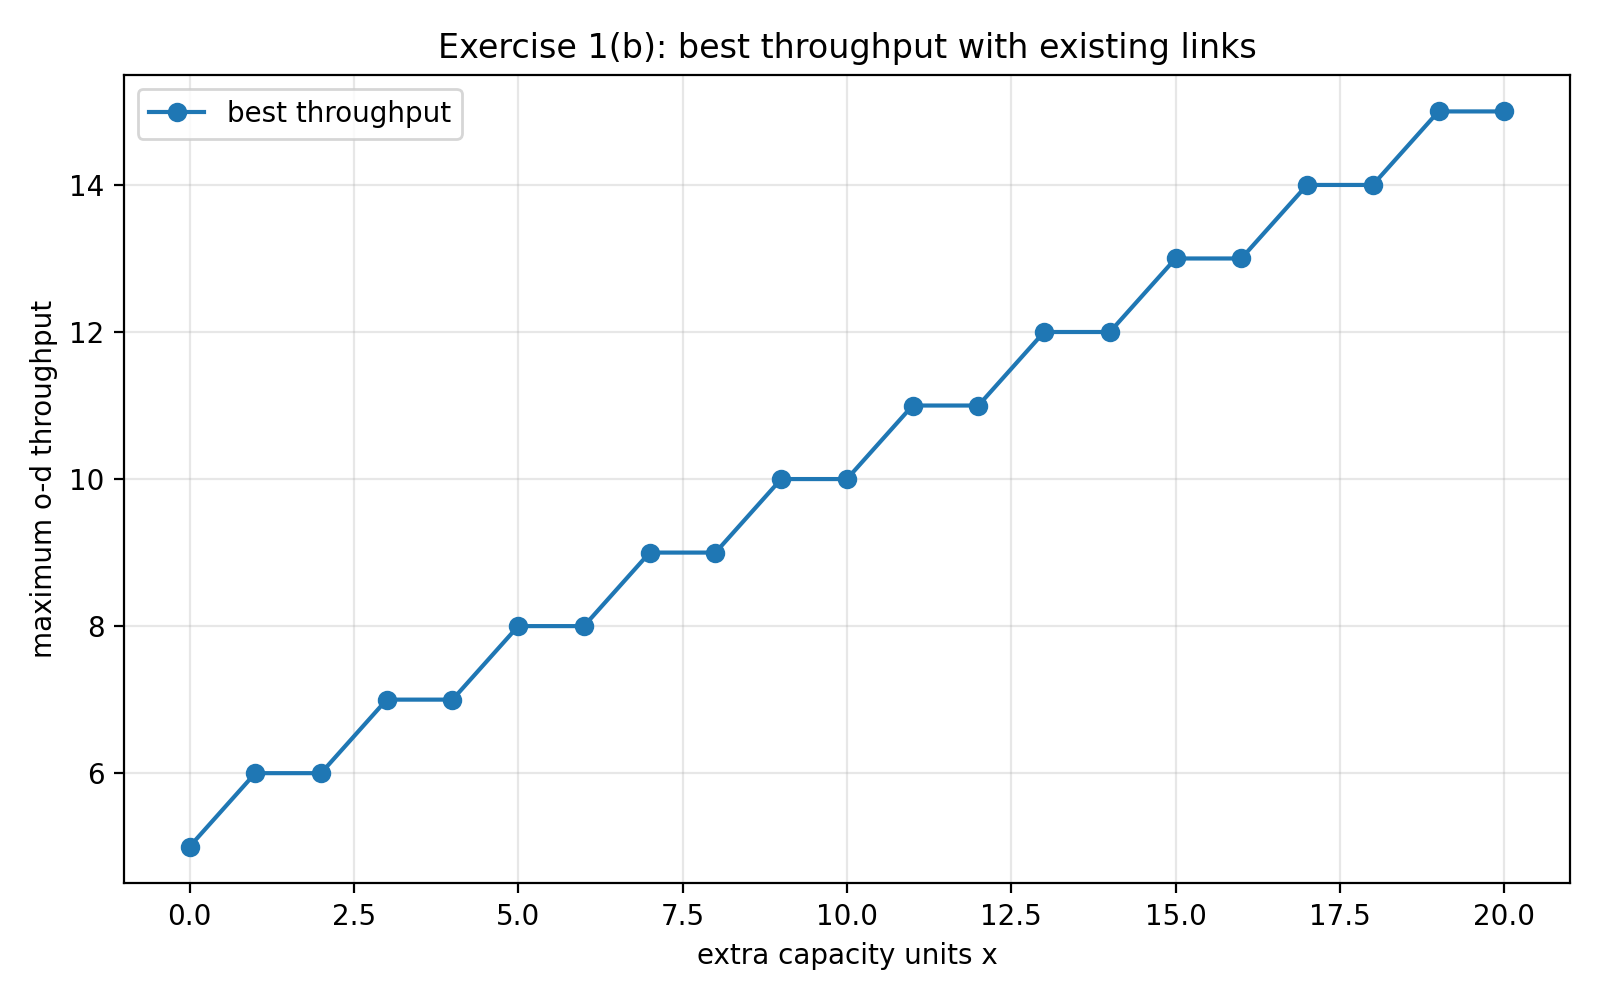
\includegraphics[width=0.75\textwidth]{figures/problem1_b_throughput.png}
\caption{Optimal throughput on the six existing links for integer budgets \(x\ge0\).}
\label{fig:exercise1-b-throughput}
\end{figure}

\subsection*{Adding one new link}

Part 1(c) permits one new directed arc \(e_7\) of initial capacity \(1\),
except that the direct source-to-sink arc \(o\to d\) is explicitly
forbidden. There are \(13\) admissible missing directed arcs between
distinct nodes. The search checks each admissible candidate and the
integer-capacity allocations, as well as a separate min-cost-flow
verification.

A link that is optimal for \emph{every} integer budget is
\(e_7:o\to c\). For \(x=2k+r\), with \(r\in\{0,1\}\), an optimal
allocation is \(y_5=y_7=k\), \(y_6=r\), with all remaining increments
zero. With the new base link of capacity \(1\), the resulting throughput is
\[
T_c(x)=5+\left\lfloor\frac{x}{2}\right\rfloor,
\qquad x\in\mathbb Z_{>0}.
\]
This design has base throughput \(5\) at \(x=0\), which is also shown
in the CSV for comparison; the stated problem requires only \(x>0\).
The values over \(x=1,\ldots,20\) are
\[
\begin{array}{c|cccccccccc}
x &1&2&3&4&5&6&7&8&9&10\\
\hline
T_c(x)&5&6&6&7&7&8&8&9&9&10
\end{array}
\]
\[
\begin{array}{c|cccccccccc}
x &11&12&13&14&15&16&17&18&19&20\\
\hline
T_c(x)&10&11&11&12&12&13&13&14&14&15
\end{array}
\]

To prove that no other legal added link can do better, consider cuts
\(S_1=\{o\}\) and \(S_3=\{o,a,b,c\}\). Their original capacities
are \(4\) and \(5\), and their crossing-edge sets are disjoint. Any
new arc other than \(o\to d\) can cross \emph{at most one} of these
cuts. Therefore, after adding its one unit of base capacity and allocating
\(x\) further units, the sum of the two cut capacities is at most
\(4+5+1+x=10+x\). Both cuts must carry the same throughput \(F\), so
\(2F\le10+x\), hence
\(F\le5+\lfloor x/2\rfloor\). The \(o\to c\) construction attains
this bound for every integer budget.

\begin{figure}[h]
\centering
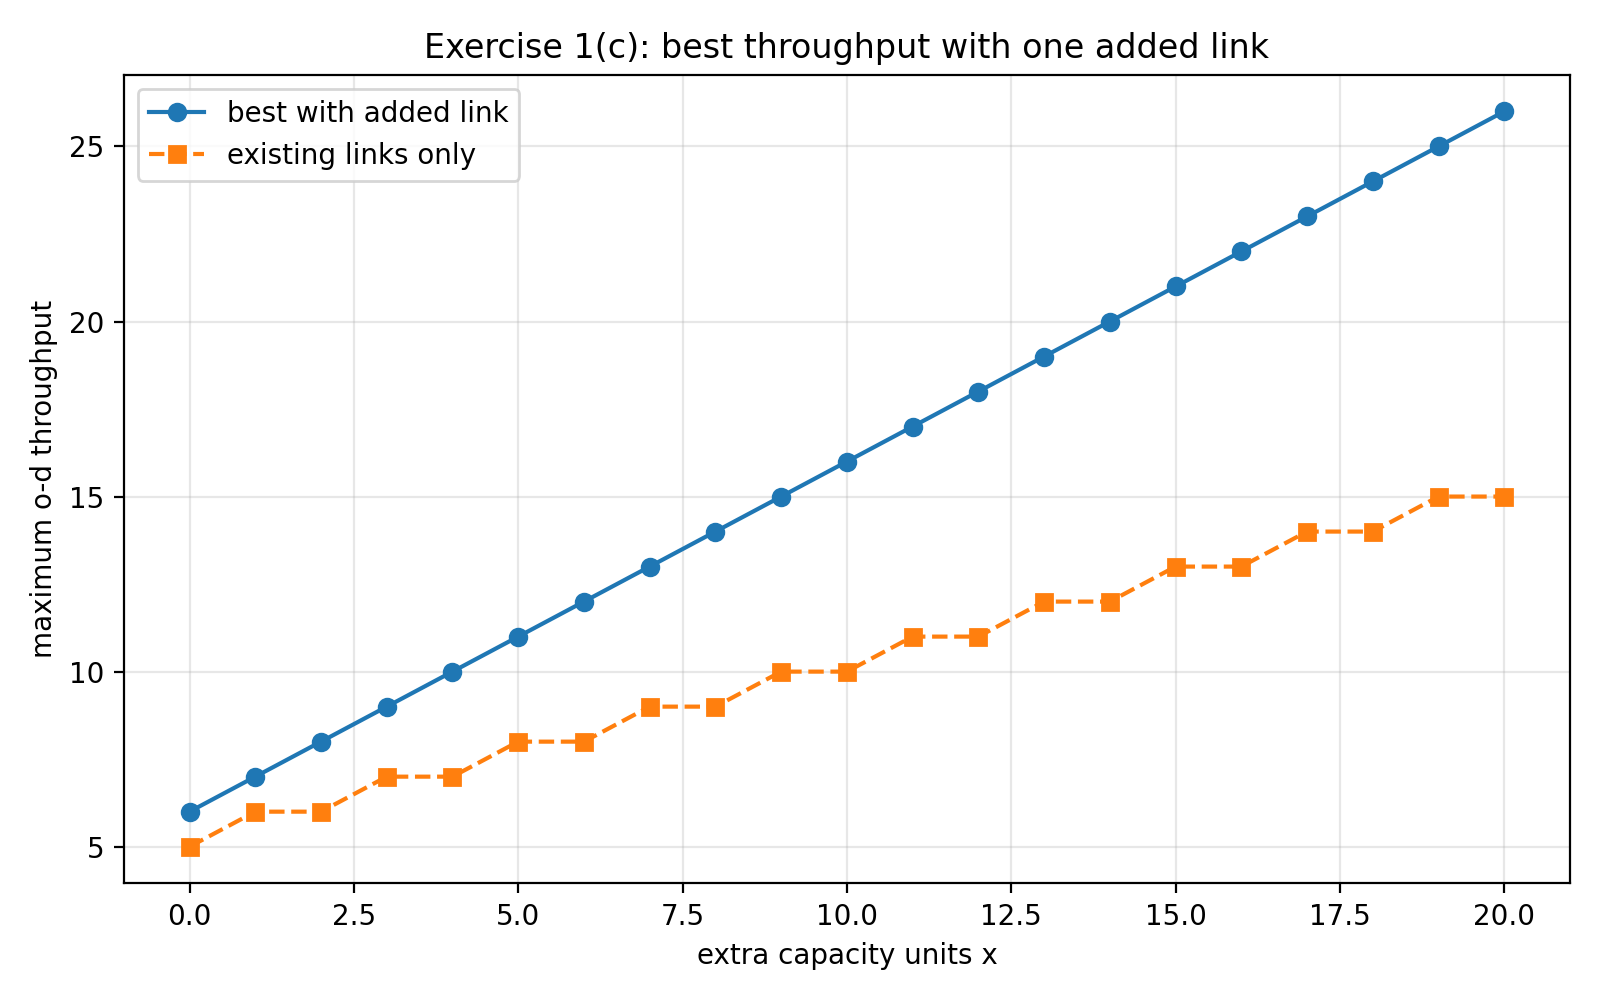
\includegraphics[width=0.75\textwidth]{figures/problem1_c_added_link_throughput.png}
\caption{Optimal legal new-link design compared with existing-link augmentation,
for integer \(x>0\).}
\label{fig:exercise1-c-throughput}
\end{figure}

The new-link design improves throughput by exactly one unit compared with
part 1(b) for every integer budget. Other added links can tie for some
budgets, but \(o\to c\) is consistently optimal and never uses the
prohibited direct \(o\to d\) arc.

\section{Exercise 2 -- Katz centrality and PageRank}

The graph was reconstructed as a simple undirected graph on
\(\{n_1,\ldots,n_{15}\}\). No visually ambiguous edges were marked in the
reconstruction. The assumed edge set is
\[
\begin{aligned}
E=\{&
n_1n_2,n_1n_3,n_1n_4,n_1n_5,n_1n_6,
n_2n_3,n_2n_4,n_2n_5,n_2n_6,\\
&n_3n_4,n_3n_5,n_3n_6,
n_4n_5,n_4n_6,n_5n_6,
n_6n_{15},n_6n_7,\\
&n_7n_8,n_8n_9,
n_9n_{10},n_9n_{11},n_9n_{12},n_9n_{13},n_9n_{14}\}.
\end{aligned}
\]
Thus the graph has \(15\) nodes and \(24\) undirected edges. In particular,
\(\{n_1,\ldots,n_6\}\) form a clique, node \(n_6\) connects this clique to
\(n_7\) and \(n_{15}\), and node \(n_9\) is the center of a star attached
through the path \(n_6-n_7-n_8-n_9\).

\subsection*{Katz centrality}

Let $W$ be the adjacency matrix of the reconstructed undirected graph and let
$\mu$ be the uniform intrinsic centrality vector, with $\mu_i=1/15$ for every node $i$. Katz centrality was computed
from
\[
x=(I-\beta W)^{-1}\mu .
\]
For \(\beta=0.15\), the largest eigenvalue of \(W\) is
\(\lambda_{\max}(W)=5.0710614673\), so
\[
\frac{1}{\lambda_{\max}(W)}=0.1971973731.
\]
The spectral condition \(\beta<1/\lambda_{\max}(W)\) is therefore satisfied.
The resulting Katz values are shown in Table~\ref{tab:exercise2-katz}; the same
values are plotted in Figure~\ref{fig:exercise2-katz}.

\begin{table}[h]
\centering
\begin{tabular}{c|c|c|c}
\hline
Rank & Node & Degree & Katz\\
\hline
1 & \(n_6\) & 7 & 0.3177933766\\
2 & \(n_1\) & 5 & 0.2858391829\\
2 & \(n_2\) & 5 & 0.2858391829\\
2 & \(n_3\) & 5 & 0.2858391829\\
2 & \(n_4\) & 5 & 0.2858391829\\
2 & \(n_5\) & 5 & 0.2858391829\\
7 & \(n_9\) & 6 & 0.1498337716\\
8 & \(n_7\) & 2 & 0.1306464788\\
9 & \(n_{15}\) & 1 & 0.1143356732\\
10 & \(n_8\) & 2 & 0.1087387042\\
11 & \(n_{10}\) & 1 & 0.0891417324\\
11 & \(n_{11}\) & 1 & 0.0891417324\\
11 & \(n_{12}\) & 1 & 0.0891417324\\
11 & \(n_{13}\) & 1 & 0.0891417324\\
11 & \(n_{14}\) & 1 & 0.0891417324\\
\hline
\end{tabular}
\caption{Katz centrality for \(\beta=0.15\).}
\label{tab:exercise2-katz}
\end{table}

\begin{figure}[h]
\centering
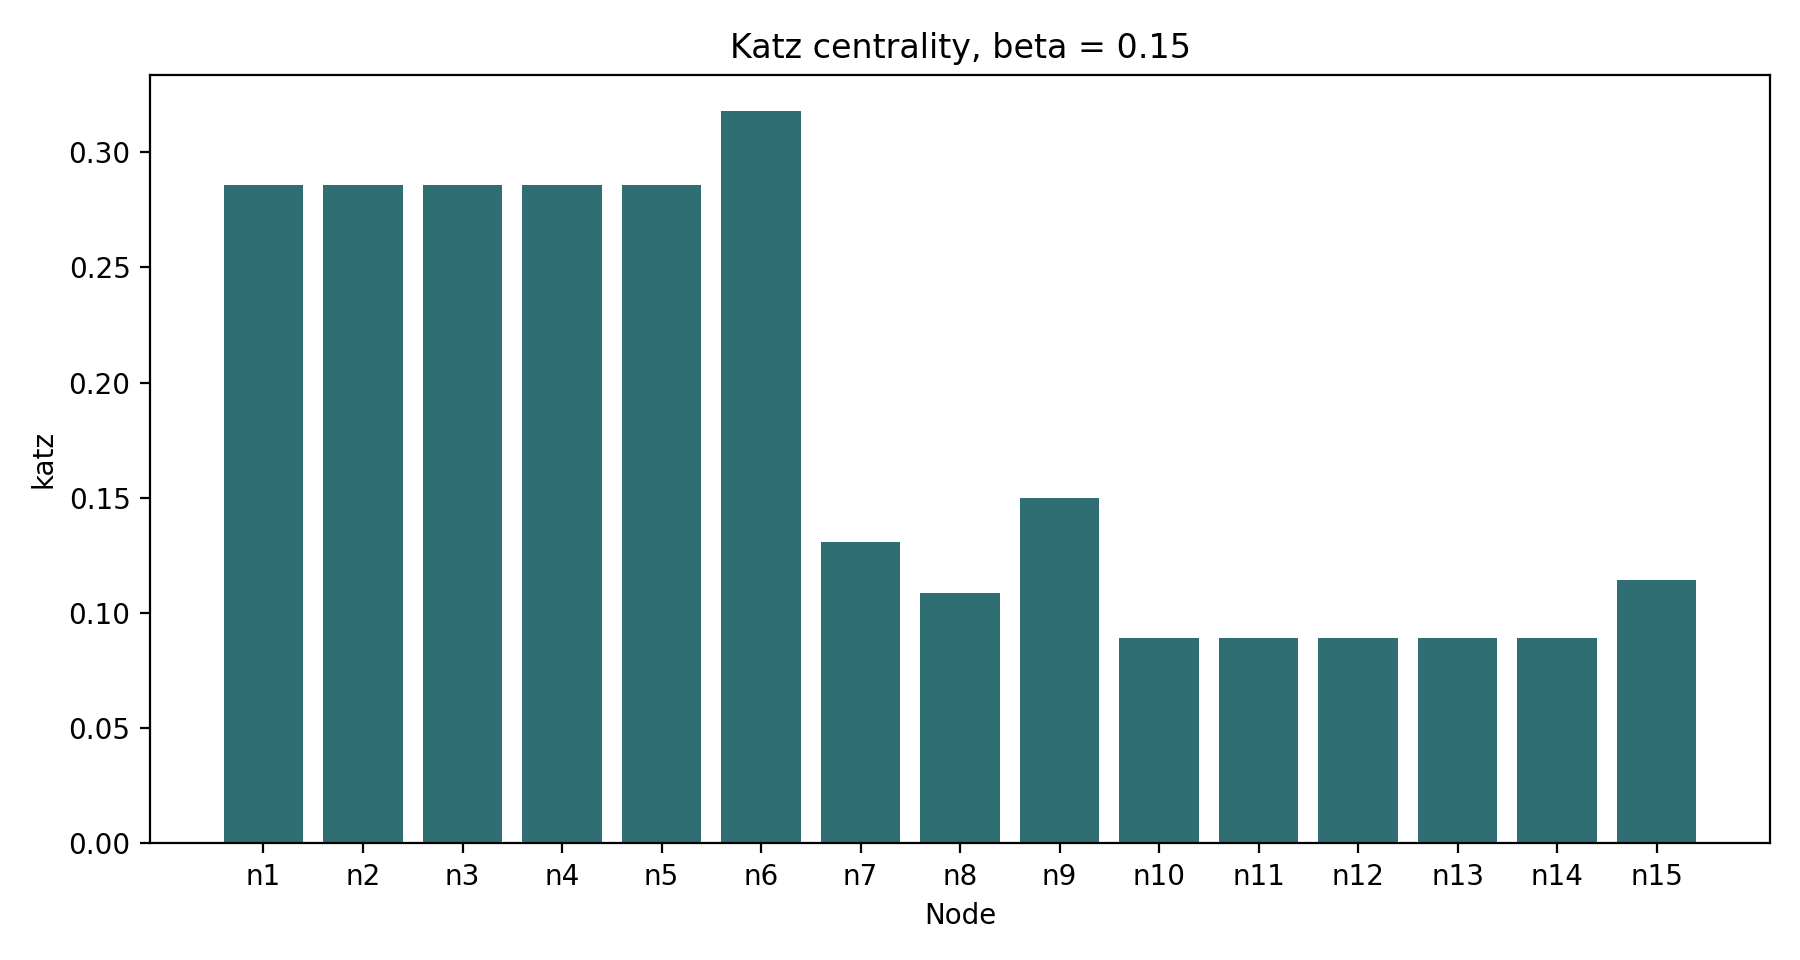
\includegraphics[width=0.75\textwidth]{figures/problem2_katz.png}
\caption{Katz centrality for the reconstructed graph with \(\beta=0.15\).}
\label{fig:exercise2-katz}
\end{figure}

\subsection*{Distributed PageRank}

For PageRank, each node iterates the distributed update
\[
x_i(t+1)=(1-\beta)\mu_i+\beta\sum_{j\in N(i)}
\frac{x_j(t)}{\deg(j)} .
\]
The distributed algorithm is:

\begin{enumerate}
    \item Initialize each node with $x_i(0)=\mu_i$.
    \item At iteration $t$, each node $j$ sends $x_j(t)/\deg(j)$ to all its neighbors.
    \item Each node $i$ sums the received messages from its neighbors.
    \item Each node updates its value using
    \[
    x_i(t+1)=(1-\beta)\mu_i+\beta\sum_{j\in N(i)}\frac{x_j(t)}{\deg(j)}.
    \]
    \item The process stops when $\|x(t+1)-x(t)\|_1$ is below the chosen tolerance.
\end{enumerate}
Equivalently, each node \(j\) sends the normalized quantity
\(x_j(t)/\deg(j)\) to each neighbor. Hence node \(i\) only needs, from each
neighbor \(j\), the current PageRank value \(x_j(t)\) and the neighbor degree
\(\deg(j)\), or directly the already normalized message \(x_j(t)/\deg(j)\).
It then sums these incoming neighbor messages and adds its intrinsic term
\((1-\beta)\mu_i\).

With \(\beta=0.15\), tolerance \(10^{-12}\), and uniform \(\mu\), the method
converged in \(15\) iterations, with final \(L^1\) difference
\(2.011\cdot 10^{-13}\). The PageRank values are reported in
Table~\ref{tab:exercise2-pagerank}; Figure~\ref{fig:exercise2-pagerank} shows
the corresponding plot.

\begin{table}[h]
\centering
\begin{tabular}{c|c|c|c}
\hline
Rank & Node & Degree & PageRank\\
\hline
1 & \(n_9\) & 6 & 0.1059574692\\
2 & \(n_6\) & 7 & 0.0801149613\\
3 & \(n_1\) & 5 & 0.0663447907\\
3 & \(n_2\) & 5 & 0.0663447907\\
3 & \(n_3\) & 5 & 0.0663447907\\
3 & \(n_4\) & 5 & 0.0663447907\\
3 & \(n_5\) & 5 & 0.0663447907\\
8 & \(n_8\) & 2 & 0.0640546671\\
9 & \(n_7\) & 2 & 0.0631875159\\
10 & \(n_{10}\) & 1 & 0.0593156034\\
10 & \(n_{11}\) & 1 & 0.0593156034\\
10 & \(n_{12}\) & 1 & 0.0593156034\\
10 & \(n_{13}\) & 1 & 0.0593156034\\
10 & \(n_{14}\) & 1 & 0.0593156034\\
15 & \(n_{15}\) & 1 & 0.0583834158\\
\hline
\end{tabular}
\caption{Distributed PageRank for \(\beta=0.15\).}
\label{tab:exercise2-pagerank}
\end{table}

\begin{figure}[h]
\centering
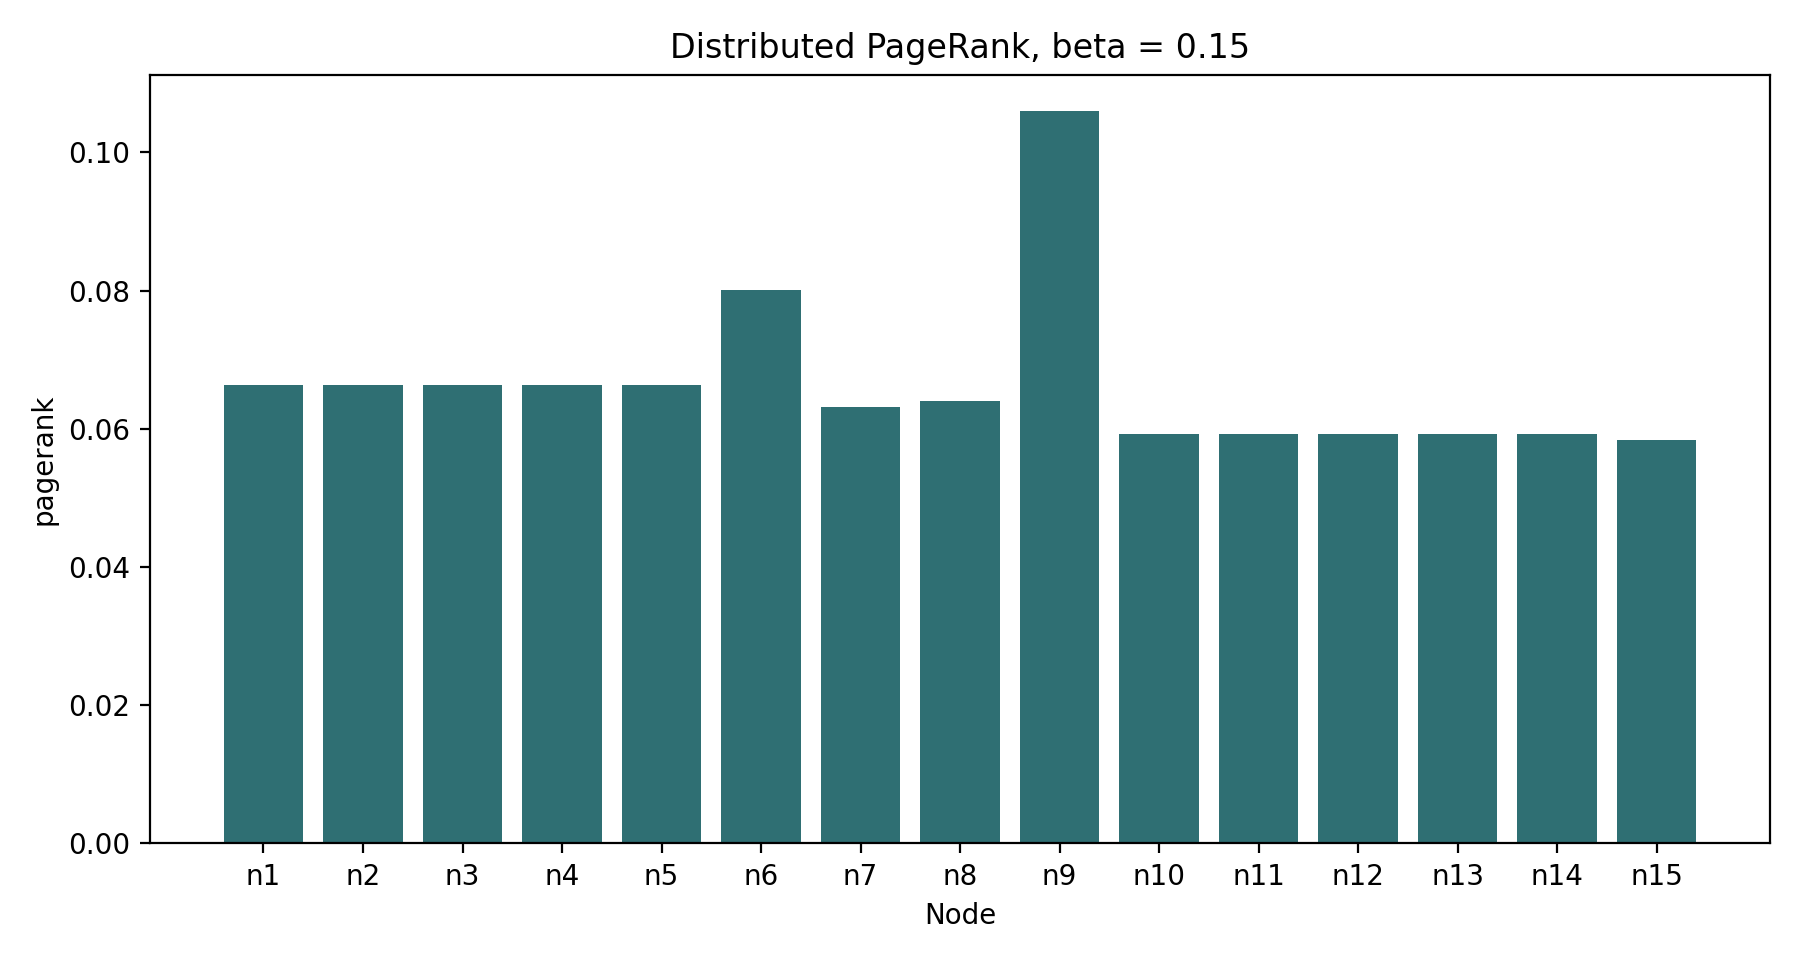
\includegraphics[width=0.75\textwidth]{figures/problem2_pagerank_beta015.png}
\caption{Distributed PageRank for the reconstructed graph with \(\beta=0.15\).}
\label{fig:exercise2-pagerank}
\end{figure}

\subsection*{Comparison of \(n_6\) and \(n_9\)}

The two nodes have different behavior under Katz centrality and PageRank:
\[
\begin{array}{c|c|c|c|l}
\hline
\text{node} & \text{degree} & \text{Katz} & \text{PageRank} & \text{neighbors}\\
\hline
n_6 & 7 & 0.3177933766 & 0.0801149613
& n_1,n_2,n_3,n_4,n_5,n_7,n_{15}\\
n_9 & 6 & 0.1498337716 & 0.1059574692
& n_8,n_{10},n_{11},n_{12},n_{13},n_{14}\\
\hline
\end{array}
\]
Katz ranks \(n_6\) above \(n_9\). This is because Katz centrality counts raw
walk contributions, and \(n_6\) is embedded in the dense six-node clique while
also acting as the bridge toward the path and \(n_{15}\). PageRank ranks
\(n_9\) above \(n_6\). The reason is the degree normalization in the PageRank
update: the degree-one leaves \(n_{10},\ldots,n_{14}\) send all their PageRank
mass to \(n_9\), whereas the clique nodes adjacent to \(n_6\) split their mass
among five neighbors.

\subsection*{PageRank sensitivity to \(\beta\)}

The PageRank comparison between \(n_6\) and \(n_9\) was repeated for
\(\beta\in\{0,1/4,1/2,3/4,1\}\). The results are shown in
Table~\ref{tab:exercise2-beta}. At \(\beta=0\), only the uniform intrinsic
centrality matters, so all nodes have PageRank \(1/15=0.0666666667\). At
\(\beta=1\), the score is determined only by the graph random-walk structure. For $\beta=1$, the PageRank recursion becomes the simple random-walk iteration.
Since the reconstructed graph is connected and non-bipartite, the random walk has a
unique stationary distribution
\[
\pi_i=\frac{\deg(i)}{2|E|}.
\]
Here $|E|=24$, so
\[
PR(n_6)=\frac{7}{48}, \qquad PR(n_9)=\frac{6}{48},
\]
and therefore
\[
PR(n_6)-PR(n_9)=\frac{1}{48}\approx 0.020833.
\]

\begin{table}[h]
\centering
\begin{tabular}{c|c|c|c|c}
\hline
\(\beta\) & \(PR(n_6)\) & \(PR(n_9)\) & \(PR(n_6)-PR(n_9)\) & Iterations\\
\hline
0.00 & 0.0666666667 & 0.0666666667 & 0.0000000000 & 1\\
0.25 & 0.0875066385 & 0.1269777272 & -0.0394710887 & 20\\
0.50 & 0.1014039855 & 0.1666925466 & -0.0652885611 & 38\\
0.75 & 0.1106044872 & 0.1911159378 & -0.0805114506 & 88\\
1.00 & 0.1458333333 & 0.1250000000 & 0.0208333333 & 1083\\
\hline
\end{tabular}
\caption{PageRank sensitivity for nodes \(n_6\) and \(n_9\).}
\label{tab:exercise2-beta}
\end{table}

\begin{figure}[h]
\centering
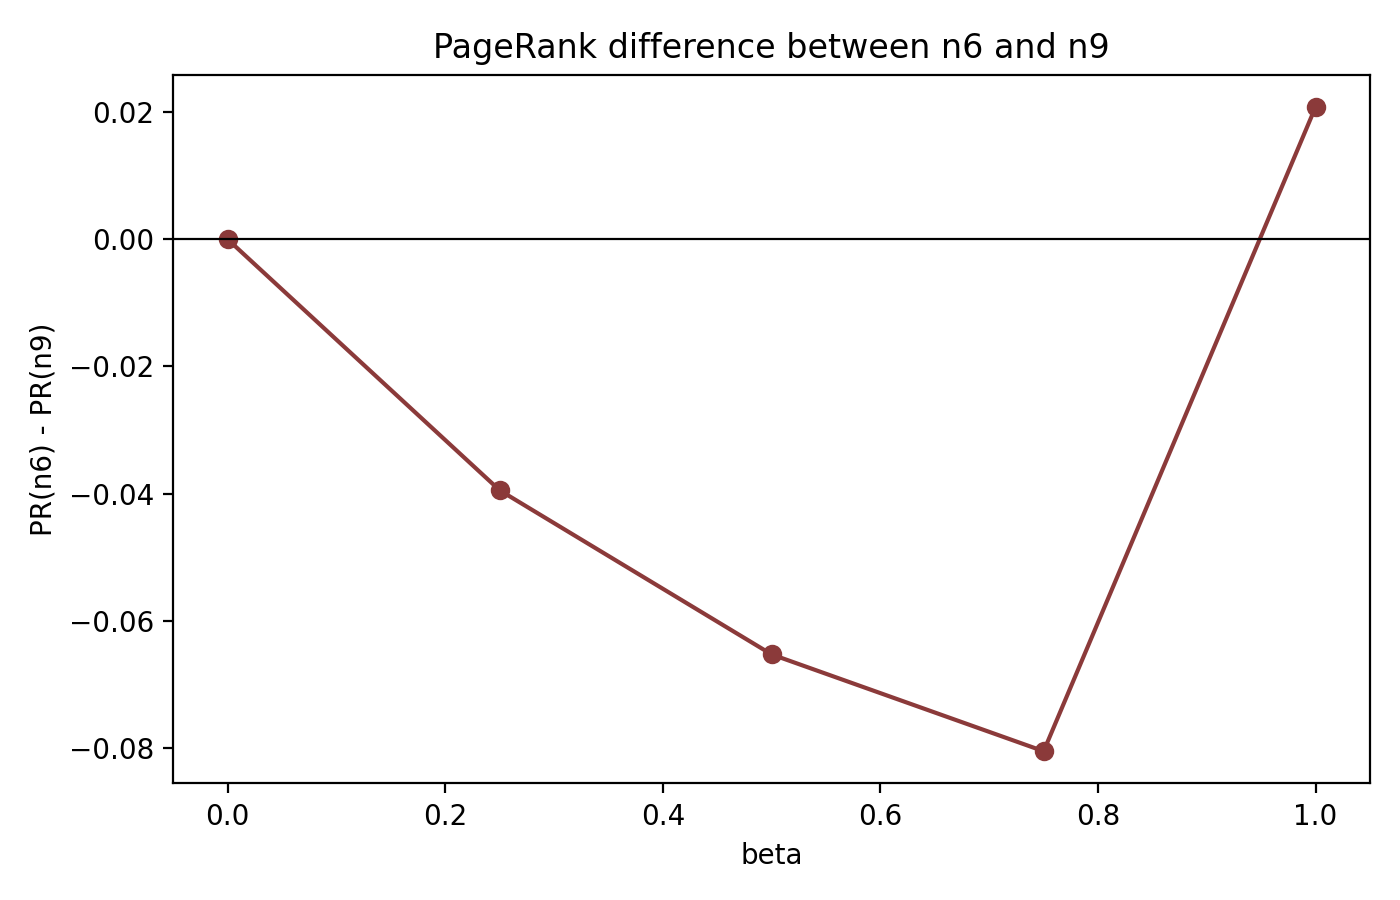
\includegraphics[width=0.75\textwidth]{figures/problem2_pagerank_difference_beta.png}
\caption{Difference \(PR(n_6)-PR(n_9)\) as a function of \(\beta\).}
\label{fig:exercise2-beta-difference}
\end{figure}

The tested sequence \(PR(n_6)-PR(n_9)\) is not monotone in \(\beta\): it first
decreases from \(0\) to \(-0.0805114506\), then increases to
\(0.0208333333\) at \(\beta=1\).

\section{Exercise 3 -- Traffic assignment}

\noindent\textbf{Data provenance.} The traffic input matrices and corresponding
numerical values below come from the four \texttt{.mat} files currently stored
in the project repository. The assignment continues to name the same files in
2026/27, but their latest contents must be compared with the official course
files before submission. The figures and numbers in this section are retained
from the prior project until that check is possible.


The traffic network is a directed graph with \(17\) nodes and \(28\) directed
links. The data are loaded from the four matrix files: the measured flow
vector \(f\), the capacity vector \(C\), the incidence matrix \(B\), and the
free-flow travel-time vector \(l\). The incidence matrix has one column per
link and one row per node. In each link column, \(+1\) marks the tail node and
\(-1\) marks the head node. Reconstructing the directed links from \(B\)
therefore gives exactly the \(28\) links used in the graph computations.

For link \(e\), the travel-time function is
\[
\tau_e(f_e)=\frac{l_e}{1-f_e/C_e}, \qquad 0\leq f_e<C_e.
\]
In the convex programs below, the numerical constraint
\[
0\leq f_e\leq 0.999 C_e
\]
is imposed on every link. This numerical upper bound keeps the optimization strictly inside the domain
$f_e<C_e$, where the delay function is finite. After solving the optimization
problems, the maximum utilization $f_e/C_e$ was checked to ensure that the
solution is not artificially determined by the numerical cap.

All convex optimization problems were solved with CVXPY using the same flow
conservation constraints and non-negativity/capacity constraints. Solver status,
objective value, and feasibility were checked for each optimization problem. The numerical results were obtained with CVXPY using the solver \texttt{clarabel}, with the default solver tolerances unless otherwise specified. After each solve, the residual \(\|Bf-\nu^{\mathrm{new}}\|_2\), the objective value, the solver status, and the maximum utilization \(\max_e f_e/C_e\) were checked. In all reported optimization problems the solver status was \texttt{optimal}, and the utilization check confirmed that the artificial bound \(f_e\leq 0.999C_e\) was not determining the solution.

\subsection*{Shortest path and maximum flow}

Using the free-flow times \(l_e\) as edge weights, the shortest path from node
\(1\) to node \(17\) is
\[
1\to 2\to 3\to 9\to 13\to 17,
\]
using links
\[
1,\ 2,\ 12,\ 9,\ 25.
\]
The total free-flow travel time on this path is \(0.559833\).

Using the capacities \(C_e\), the maximum \(1\)-to-\(17\) flow is
\[
22448.000000.
\]

\subsection*{Exogenous inflow vector}

The original node imbalance is computed from the measured flow by
\[
\nu = Bf.
\]
For the optimization problems, only the net source inflow at node \(1\) and
the corresponding sink outflow at node \(17\) are kept:
\[
\nu^{\mathrm{new}}_1=\nu_1=16806,\qquad
\nu^{\mathrm{new}}_{17}=-16806,
\]
and all other entries are set to zero. Table~\ref{tab:exercise3-nu} reports
both vectors.

\begin{table}[h]
\centering
\begin{tabular}{c|r|r}
\hline
Node & \(\nu=Bf\) & \(\nu^{\mathrm{new}}\)\\
\hline
1 & 16806 & 16806\\
2 & 8570 & 0\\
3 & 19448 & 0\\
4 & 4957 & 0\\
5 & -746 & 0\\
6 & 4768 & 0\\
7 & 413 & 0\\
8 & -2 & 0\\
9 & -5671 & 0\\
10 & 1169 & 0\\
11 & -5 & 0\\
12 & -7131 & 0\\
13 & -380 & 0\\
14 & -7412 & 0\\
15 & -7810 & 0\\
16 & -3430 & 0\\
17 & -23544 & -16806\\
\hline
\end{tabular}
\caption{Original and reduced exogenous inflow vectors.}
\label{tab:exercise3-nu}
\end{table}

\subsection*{Social optimum}

The social optimum minimizes total travel time:
\[
\begin{aligned}
\min_f \quad & \sum_e f_e \tau_e(f_e)\\
\text{s.t.}\quad & Bf=\nu^{\mathrm{new}},\\
&0\leq f\leq 0.999C .
\end{aligned}
\]
For the given delay function, the equivalent convex objective used in CVXPY is
\[
\sum_e \left(\frac{l_e C_e}{1-f_e/C_e}-l_e C_e\right).
\]
The solver status was \(\mathrm{optimal}\). The optimal total travel time was
\[
26142.669150.
\]

\subsection*{Wardrop equilibrium}

The Wardrop equilibrium is obtained by minimizing the Beckmann potential
\[
\begin{aligned}
\min_f \quad & \sum_e -l_e C_e\log(1-f_e/C_e)\\
\text{s.t.}\quad & Bf=\nu^{\mathrm{new}},\\
&0\leq f\leq 0.999C .
\end{aligned}
\]
The solver status was again \(\mathrm{optimal}\). The total travel time at the
Wardrop equilibrium was
\[
26495.321759.
\]
Compared with the social optimum, this gives the price of anarchy
\[
\frac{26495.321759}{26142.669150}=1.013490.
\]
Thus the selfish-routing equilibrium has about \(1.349\%\) larger total travel
time than the social optimum.

\subsection*{Marginal-cost tolls}

To decentralize the social optimum, marginal-cost tolls are set to
\[
\omega_e=f^{\star}_e \tau'_e(f^{\star}_e),
\qquad
\tau'_e(f_e)=\frac{l_e/C_e}{(1-f_e/C_e)^2}.
\]
The tolled Wardrop problem minimizes
\[
\sum_e -l_e C_e\log(1-f_e/C_e)+\sum_e \omega_e f_e
\]
under the same flow-conservation and capacity constraints. The tolled Wardrop
solver status was \(\mathrm{optimal}\), and the verification error was
\[
\|f^{\mathrm{tolled}}-f^\star\|_2=2.993561\cdot 10^{-1}.
\]
Since the flows are on the order of thousands of vehicles, this absolute norm is
small. To make the comparison scale-independent, the relative error
\[
\frac{\|f^{tolled}-f^\star\|_2}{\|f^\star\|_2}
\]
was also checked. In the reported run, the relative discrepancy was approximately
\[
\frac{\|f^{\mathrm{tolled}}-f^\star\|_2}{\|f^\star\|_2}
\simeq 1.33\cdot 10^{-5},
\]
which is negligible at the scale of the reported flows. This confirms that the marginal-cost tolls recover the social optimum up to solver tolerance. 
\subsection*{Additional-delay objective and tolls}

The additional-delay objective subtracts free-flow time from each link cost:
\[
\psi_e(f_e)=f_e(\tau_e(f_e)-l_e).
\]
The optimization problem is
\[
\begin{aligned}
\min_f \quad & \sum_e \psi_e(f_e)\\
\text{s.t.}\quad & Bf=\nu^{\mathrm{new}},\\
&0\leq f\leq 0.999C .
\end{aligned}
\]
The optimum solver status was \(\mathrm{optimal}\), with objective value
\[
15350.353857.
\]
The tolls that decentralize this optimum are
\[
\omega^{\mathrm{add}}_e
=\psi'_e(f^{\star,\mathrm{add}}_e)-\tau_e(f^{\star,\mathrm{add}}_e)
=-l_e+f^{\star,\mathrm{add}}_e\tau'_e(f^{\star,\mathrm{add}}_e).
\]
The corresponding tolled Wardrop solver status was \(\mathrm{optimal}\), and
\[
\|f^{\mathrm{tolled,add}}-f^{\star,\mathrm{add}}\|_2
=5.658613\cdot 10^{-1}.
\]
This is again small relative to the link flows. In relative terms,
\[
\frac{\|f^{\mathrm{tolled,add}}-f^{\star,\mathrm{add}}\|_2}{\|f^{\star,\mathrm{add}}\|_2}
\simeq 2.51\cdot 10^{-5},
\]
so the additional-delay tolls recover the additional-delay optimum within numerical accuracy.

\begin{table}[h]
\centering
\begin{tabular}{l|r}
\hline
Quantity & Value\\
\hline
Social optimum total travel time & 26142.669150\\
Wardrop total travel time & 26495.321759\\
Price of anarchy & 1.013490\\
Additional-delay optimum objective & 15350.353857\\
\(\|f^{\mathrm{tolled}}-f^\star\|_2\) & \(2.993561\cdot 10^{-1}\)\\
\(\|f^{\mathrm{tolled,add}}-f^{\star,\mathrm{add}}\|_2\) &
\(5.658613\cdot 10^{-1}\)\\
\(\|f^{\mathrm{tolled}}-f^\star\|_2 / \|f^\star\|_2\) & \(1.33\cdot 10^{-5}\) \\
\(\|f^{\mathrm{tolled,add}}-f^{\star,\mathrm{add}}\|_2 / \|f^{\star,\mathrm{add}}\|_2\) & \(2.51\cdot 10^{-5}\) \\
\hline
\end{tabular}
\caption{Main optimization and verification results for Exercise 3.}
\label{tab:exercise3-summary}
\end{table}

\begin{table}[h]
\centering
\scriptsize
\begin{tabular}{c|r|r}
\hline
Edge & \(\omega\) & \(\omega^{\mathrm{add}}\)\\
\hline
1 & 1.973436 & 1.843996\\
2 & 0.193184 & 0.110524\\
3 & 0.049432 & -0.070804\\
4 & 0.100106 & -0.066454\\
5 & 1.512756 & 1.367481\\
6 & 0.483666 & 0.406893\\
7 & 0.112309 & 0.027030\\
8 & 0.059648 & 0.008671\\
9 & 0.271745 & 0.101759\\
10 & 0.008287 & -0.093639\\
11 & 0.000000 & -0.106670\\
12 & 0.067438 & -0.059339\\
13 & 0.000000 & -0.112330\\
14 & 0.120075 & -0.034066\\
15 & 0.498195 & 0.369956\\
16 & 0.084654 & 0.017702\\
17 & 0.073394 & -0.003661\\
18 & 0.019181 & -0.035492\\
19 & 0.001514 & -0.031226\\
20 & 0.013113 & -0.024622\\
21 & 0.067738 & 0.009238\\
22 & 0.257081 & 0.123439\\
23 & 0.066941 & -0.020805\\
24 & 0.000000 & -0.054167\\
25 & 0.391850 & 0.272065\\
26 & 0.269515 & 0.228422\\
27 & 0.147694 & 0.025865\\
28 & 0.597989 & 0.423527\\
\hline
\end{tabular}
\caption{Marginal-cost tolls for the social optimum and tolls for the
additional-delay optimum.}
\label{tab:exercise3-tolls}
\end{table}




Some tolls for the additional-delay objective are negative. This is not a numerical
error. For the objective
\[
\psi_e(f_e)=f_e(\tau_e(f_e)-l_e),
\]
the decentralizing toll is
\[
\omega_e^{add}=\psi'_e(f_e^{\star,add})-\tau_e(f_e^{\star,add})
= -l_e + f_e^{\star,add}\tau'_e(f_e^{\star,add}).
\]
Thus, links whose congestion externality is small relative to their free-flow time
can receive a negative toll. This can be interpreted as a subsidy, or equivalently
as a toll offset.

\section{Conclusion}

Exercise 1 confirmed that the minimum cut capacity and maximum flow are both \(4\).
On the original links the optimal throughput is
\(T_b(x)=4+\lfloor x/2\rfloor\), reaching \(14\) at \(x=20\).
With one permitted added link \(e_7:o\to c\), the optimal throughput is
\(T_c(x)=5+\lfloor x/2\rfloor\), reaching \(15\) at \(x=20\).
Both formulas are supported by explicit capacity allocations and cut-based upper bounds.
The direct source-to-sink link \(o\to d\) is excluded as required in 2026/27.

Exercise 2 showed that Katz centrality and PageRank emphasize different
structural roles. Katz centrality ranks \(n_6\) highest because it is embedded
in the dense clique and also connects to the rest of the graph. PageRank ranks
\(n_9\) highest for \(\beta=0.15\), because several degree-one neighbors send
all their normalized mass to \(n_9\). The sensitivity test showed that
\(PR(n_6)-PR(n_9)\) is not monotone in \(\beta\).

Exercise 3 compared routing objectives on the traffic network. The Wardrop
equilibrium has total travel time \(26495.321759\), compared with
\(26142.669150\) at the social optimum, giving a price of anarchy of
\(1.013490\). The marginal-cost tolls and the additional-delay tolls both
recover their target optima within small numerical discrepancies relative to
the scale of the link flows.

\appendix



\section{Detailed edge-flow comparison}

\begin{table}[h]
\centering
\scriptsize
\begin{tabular}{c|c|r|r|r|r|r}
\hline
Edge & Arc & \(f^\star\) & \(f^{W}\) & \(f^{\mathrm{tolled}}\) &
\(f^{\star,\mathrm{add}}\) & \(f^{\mathrm{tolled,add}}\)\\
\hline
1 & \(1\to2\) & 6569.213 & 6557.510 & 6569.053 & 6584.465 & 6584.310\\
2 & \(2\to3\) & 5809.999 & 6308.594 & 5809.976 & 5577.902 & 5578.047\\
3 & \(3\to4\) & 3046.970 & 2200.641 & 3046.966 & 3367.453 & 3367.367\\
4 & \(4\to5\) & 3046.970 & 2200.641 & 3046.966 & 3367.453 & 3367.367\\
5 & \(1\to6\) & 10236.787 & 10248.490 & 10236.947 & 10221.535 & 10221.690\\
6 & \(6\to7\) & 4666.496 & 4706.686 & 4666.565 & 4669.458 & 4669.522\\
7 & \(7\to8\) & 3061.217 & 2859.927 & 3061.219 & 3156.434 & 3156.371\\
8 & \(8\to9\) & 2595.955 & 2232.651 & 2595.958 & 2711.828 & 2711.726\\
9 & \(9\to13\) & 3104.550 & 3350.007 & 3104.548 & 2987.937 & 2987.976\\
10 & \(2\to7\) & 759.214 & 248.916 & 759.077 & 1006.563 & 1006.263\\
11 & \(3\to8\) & 0.000 & 11.665 & 0.000 & 0.000 & 0.000\\
12 & \(3\to9\) & 2763.029 & 4096.288 & 2763.010 & 2210.449 & 2210.680\\
13 & \(4\to9\) & 0.000 & 0.000 & 0.000 & 0.000 & 0.000\\
14 & \(5\to14\) & 3046.970 & 2200.641 & 3046.966 & 3367.453 & 3367.367\\
15 & \(6\to10\) & 5570.291 & 5541.804 & 5570.382 & 5552.076 & 5552.168\\
16 & \(10\to11\) & 2893.839 & 2343.349 & 2893.856 & 3084.751 & 3084.683\\
17 & \(10\to15\) & 5040.945 & 5294.130 & 5040.949 & 4986.912 & 4986.898\\
18 & \(7\to10\) & 2364.493 & 2095.675 & 2364.423 & 2519.587 & 2519.413\\
19 & \(8\to11\) & 465.262 & 638.941 & 465.260 & 444.607 & 444.645\\
20 & \(9\to12\) & 2254.434 & 2978.932 & 2254.420 & 1934.340 & 1934.430\\
21 & \(11\to12\) & 3359.102 & 2982.290 & 3359.116 & 3529.358 & 3529.328\\
22 & \(12\to13\) & 5613.535 & 5961.222 & 5613.536 & 5463.697 & 5463.758\\
23 & \(13\to14\) & 2371.991 & 2522.440 & 2371.992 & 2202.316 & 2202.404\\
24 & \(11\to15\) & 0.000 & 0.000 & 0.000 & 0.000 & 0.000\\
25 & \(13\to17\) & 6346.094 & 6788.789 & 6346.093 & 6249.318 & 6249.331\\
26 & \(14\to17\) & 5418.960 & 4723.081 & 5418.958 & 5569.769 & 5569.771\\
27 & \(15\to16\) & 5040.945 & 5294.130 & 5040.949 & 4986.912 & 4986.898\\
28 & \(16\to17\) & 5040.945 & 5294.130 & 5040.949 & 4986.912 & 4986.898\\
\hline
\end{tabular}
\caption{Edge-flow comparison for the social optimum, Wardrop equilibrium,
marginal-cost tolled Wardrop, additional-delay optimum, and additional-delay
tolled Wardrop.}
\label{tab:exercise3-flows}
\end{table}



\begin{figure}[h]
\centering
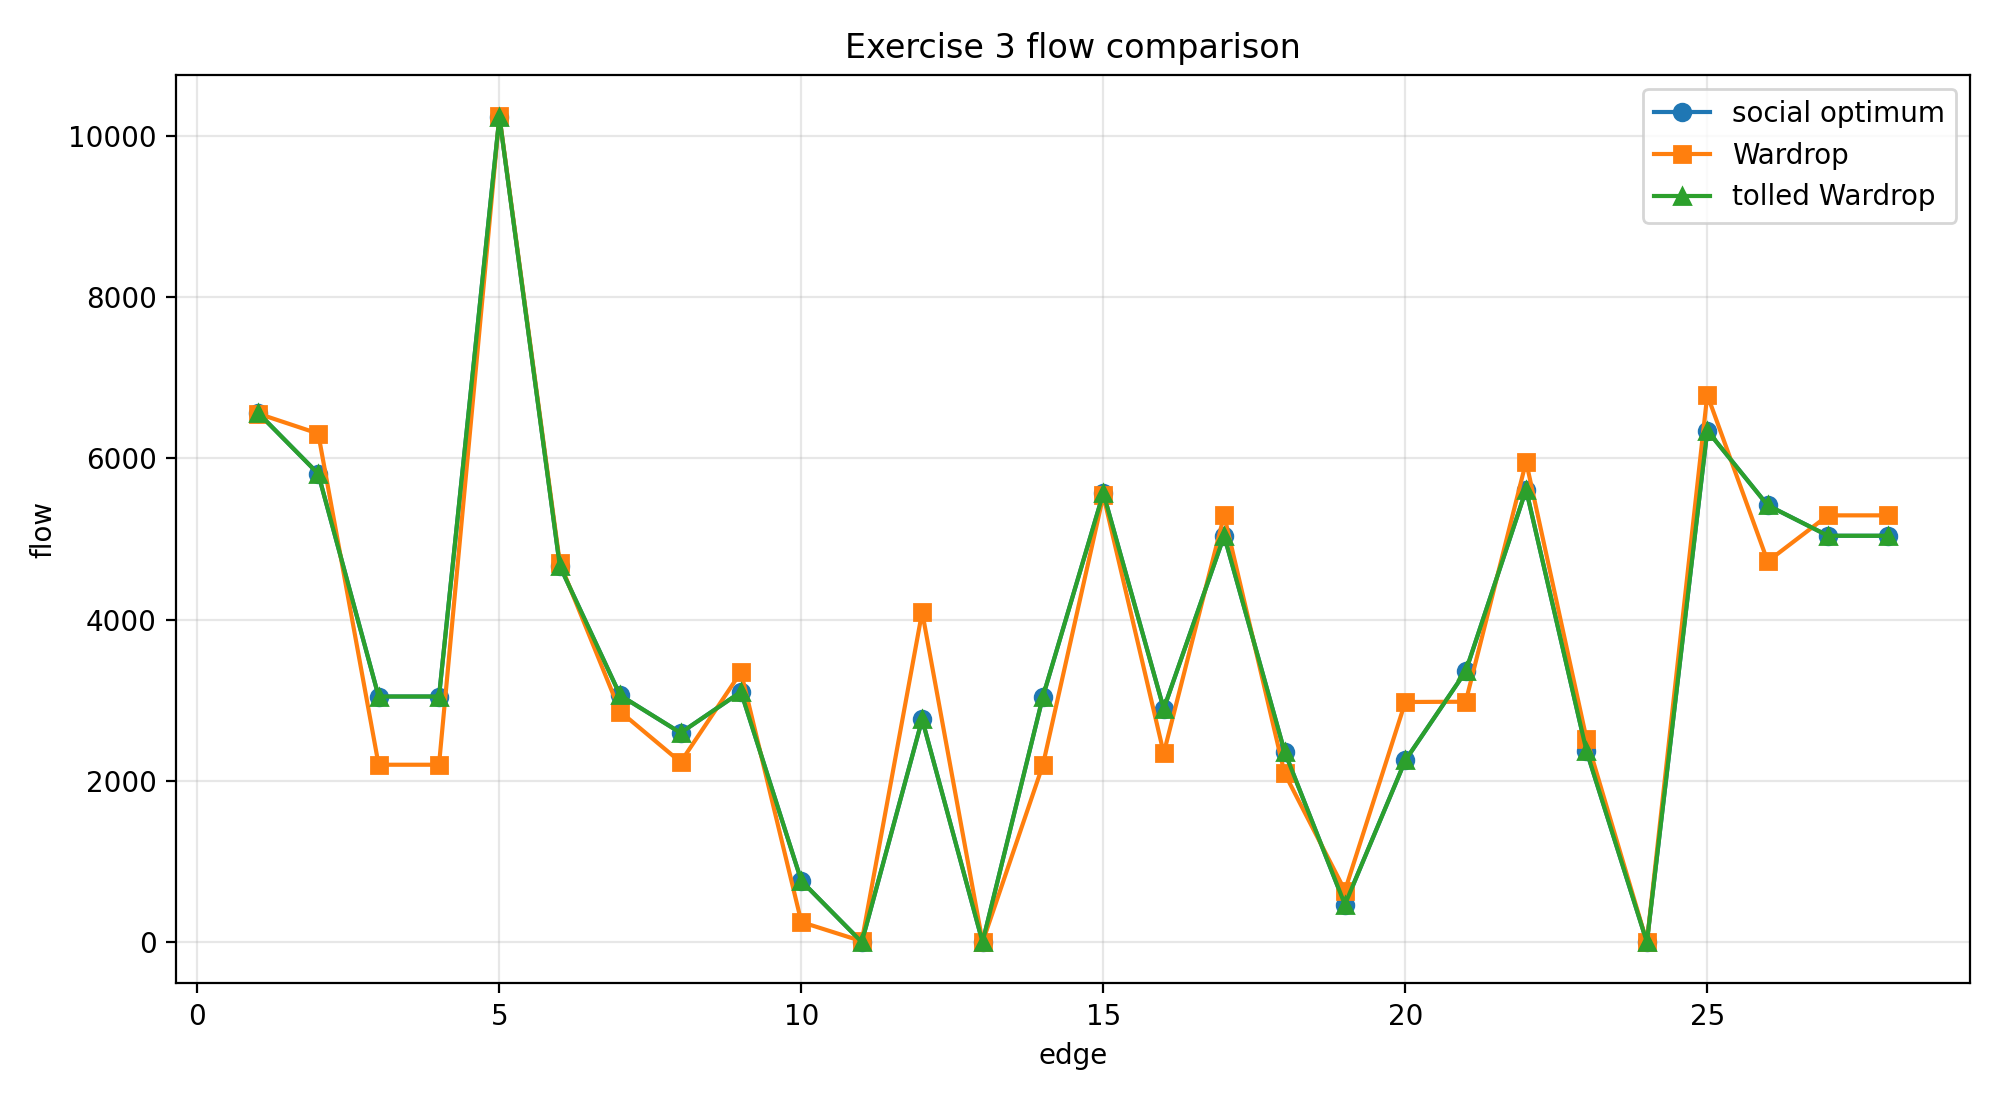
\includegraphics[width=0.8\textwidth]{figures/problem3_flow_comparison.png}
\caption{Flow comparison between the social optimum, untolled Wardrop
equilibrium, and marginal-cost tolled Wardrop equilibrium.}
\label{fig:exercise3-flow-comparison}
\end{figure}

% ------------------------------------------------------------------
% Insert after the existing Appendix A.
% This should become Appendix B if \appendix was already issued.
% ------------------------------------------------------------------

\section{Reproducibility and Numerical Verification}
\label{app:hw1-reproducibility}

This appendix summarizes the implementation choices and numerical checks used to obtain the
results in the main report. It is not meant to replace the derivations in the main text; rather, it
records the computational conventions that are useful for reproducing the tables and for defending
the modelling choices orally.

\subsection{Repository-to-report mapping}

All scripts are intended to be run from the \texttt{hw1/} directory. The following table maps each
exercise to the corresponding source file, input data, and generated outputs.

\begin{center}
\scriptsize

\begin{tabular}{p{0.10\textwidth} p{0.20\textwidth} p{0.23\textwidth} p{0.27\textwidth}}
\hline
Task & Script & Inputs & Main outputs \\
\hline
Exercise 1 &
\texttt{src/run\_problem1.py} &
Hard-coded graph with nodes $\{o,a,b,c,d\}$ and capacities $c_1,\ldots,c_6$ &
\texttt{results/problem1\_cuts.csv},
\texttt{results/problem1\_b\_results.csv},
\texttt{results/problem1\_c\_results.csv},
\texttt{figures/problem1\_b\_throughput.png},
\texttt{figures/problem1\_c\_added\_link\_throughput.png}
\\
\hline
Exercise 2 &
\texttt{src/run\_problem2.py} &
Reconstructed undirected graph from the assignment figure; uniform intrinsic centrality $\mu$ &
\texttt{results/problem2\_katz.csv},
\texttt{results/problem2\_pagerank\_beta015.csv},
\texttt{results/problem2\_pagerank\_beta\_sensitivity.csv},
\texttt{figures/problem2\_katz.png},
\texttt{figures/problem2\_pagerank\_beta015.png},
\texttt{figures/problem2\_pagerank\_difference\_beta.png}
\\
\hline
Exercise 3 &
\texttt{src/run\_problem3.py} &
\texttt{data/flow.mat},
\texttt{data/capacities.mat},
\texttt{data/traffic.mat},
\texttt{data/traveltime.mat} &
\texttt{results/problem3\_shortest\_path.csv},
\texttt{results/problem3\_maxflow.csv},
\texttt{results/problem3\_nu.csv},
\texttt{results/problem3\_social\_optimum.csv},
\texttt{results/problem3\_wardrop.csv},
\texttt{results/problem3\_tolls\_total\_travel\_time.csv},
\texttt{results/problem3\_additional\_delay.csv},
\texttt{figures/problem3\_flow\_comparison.png}
\\
\hline
\end{tabular}
\end{center}

\subsection{Numerical verification checklist}

The following checks were used to verify that the numerical outputs are consistent with the
mathematical formulation.

\begin{enumerate}
    \item \textbf{Max-flow/min-cut consistency.}
    All $o$--$d$ cuts were enumerated explicitly. The minimum cut capacity is $4$, and the
    NetworkX maximum-flow value on the same graph is also $4$. This verifies the
    max-flow/min-cut theorem on the instance used in Exercise 1.

    \item \textbf{Integer capacity augmentation.}
    For each budget $x=0,\ldots,20$, the code enumerates all nonnegative integer allocations
    of $x$ units over the candidate links and evaluates the resulting throughput through the
    cut-capacity characterization. This avoids relying on a heuristic allocation rule.

    \item \textbf{Added-link candidate set.}
    In Exercise 1(c), exactly the 13 missing directed links between distinct nodes
    other than the forbidden direct $o\to d$ link are admissible. The link
    $e_7:o\to c$ is optimal for every integer budget $x$. The max-flow/min-cut
    proof and the independently checked numerical results give
    \[
        T_c(x)=5+\left\lfloor\frac{x}{2}\right\rfloor.
    \]
    The source-side and sink-side disjoint cut bound demonstrates global optimality.

    \item \textbf{Katz admissibility.}
    Katz centrality was computed as
    \[
        x = (I-\beta W)^{-1}\mu.
    \]
    The reported value $\beta=0.15$ satisfies the spectral condition
    \[
        \beta < \frac{1}{\lambda_{\max}(W)}.
    \]
    This ensures that the Katz linear system is well-defined.

    \item \textbf{Distributed PageRank convergence.}
    PageRank was computed by the iteration
    \[
        x_i(t+1) = (1-\beta)\mu_i
        + \beta \sum_{j\in\mathcal{N}(i)}\frac{x_j(t)}{\deg(j)}.
    \]
    The stopping rule used the $\ell_1$ difference between consecutive iterates. For the
    main run with $\beta=0.15$, the tolerance was $10^{-12}$, and the reported convergence
    took 15 iterations.

    \item \textbf{Traffic-flow feasibility.}
    In Exercise 3, the incidence convention is
    \[
        B_{ve} =
        \begin{cases}
        +1, & \text{if node } v \text{ is the tail of edge } e,\\
        -1, & \text{if node } v \text{ is the head of edge } e,\\
        0, & \text{otherwise.}
        \end{cases}
    \]
    Therefore feasible flows satisfy
    \[
        Bf=\nu^{\mathrm{new}}, \qquad f\geq 0.
    \]
    The residual $\|Bf-\nu^{\mathrm{new}}\|_2$ was checked after each convex optimization.

    \item \textbf{Delay-domain protection.}
    The link delay
    \[
        \tau_e(f_e)=\frac{\ell_e}{1-f_e/C_e}
    \]
    is finite only for $f_e<C_e$. The optimization therefore uses the numerical upper bound
    \[
        0 \leq f_e \leq 0.999\,C_e.
    \]
    The maximum utilization was checked after solving, to verify that the artificial cap was
    not determining the reported optimizer.

    \item \textbf{Toll recovery checks.}
    Marginal-cost tolls recover the social optimum by solving the tolled Wardrop problem
    and comparing the resulting flow with the target optimum. The reported relative errors
    are
    \[
        \frac{\|f^{\mathrm{tolled}}-f^\star\|_2}{\|f^\star\|_2}
        \simeq 1.33\cdot 10^{-5},
        \qquad
        \frac{\|f^{\mathrm{tolled,add}}-f^{\star,\mathrm{add}}\|_2}
        {\|f^{\star,\mathrm{add}}\|_2}
        \simeq 2.51\cdot 10^{-5}.
    \]
    These discrepancies are negligible compared with the scale of the link flows.
\end{enumerate}

\subsection{Clarification on additional-delay tolls}

For the total-travel-time objective, the decentralizing toll is the standard marginal external
cost
\[
    \omega_e = f^\star_e \tau'_e(f^\star_e).
\]
For the additional-delay objective
\[
    \psi_e(f_e)=f_e(\tau_e(f_e)-\ell_e),
\]
the toll that makes the Wardrop equilibrium coincide with the corresponding system optimum is
\[
    \omega^{\mathrm{add}}_e
    =
    \psi'_e(f^{\star,\mathrm{add}}_e)
    -
    \tau_e(f^{\star,\mathrm{add}}_e)
    =
    -\ell_e
    +
    f^{\star,\mathrm{add}}_e \tau'_e(f^{\star,\mathrm{add}}_e).
\]
Hence, negative tolls in this second case are not a solver error. They mean that, relative to the
baseline private delay $\tau_e$, the decentralizing correction acts as a subsidy or offset on links
whose congestion externality is smaller than their free-flow-time term.

\section{Code and File Organization}

\begin{itemize}
    \item Homework folder: \texttt{hw1/}
    \item Official guideline PDF: \texttt{hw1/data/hw1\_en\_2026-27.pdf}.
    \item Input data for the traffic assignment exercise:
    \begin{itemize}
        \item \texttt{hw1/data/flow.mat}: measured flow vector.
        \item \texttt{hw1/data/capacities.mat}: edge-capacity vector.
        \item \texttt{hw1/data/traffic.mat}: node-link incidence matrix.
        \item \texttt{hw1/data/traveltime.mat}: free-flow travel-time vector.
    \end{itemize}
    \item Main scripts:
    \begin{itemize}
        \item \texttt{hw1/src/run\_problem1.py}: Exercise 1, cut enumeration, max-flow/min-cut check, integer capacity augmentation, added-link search, and throughput plots.
        \item \texttt{hw1/src/run\_problem2.py}: Exercise 2, graph reconstruction, Katz centrality, distributed PageRank, and beta sensitivity.
        \item \texttt{hw1/src/run\_problem3.py}: Exercise 3, shortest path, maximum flow, exogenous inflow vector, social optimum, Wardrop equilibrium, tolls, additional-delay objective, and flow-comparison plot.
    \end{itemize}
    \item Result files:
    \begin{itemize}
        \item Exercise 1: \texttt{hw1/results/problem1\_cuts.csv}, \\ \texttt{problem1\_b\_results.csv}, \texttt{problem1\_c\_results.csv}.
        \item Exercise 2: \texttt{hw1/results/problem2\_katz.csv}, \\ \texttt{problem2\_pagerank\_beta015.csv}, \texttt{problem2\_pagerank\_beta\_sensitivity.csv}.
        \item Exercise 3: \texttt{hw1/results/problem3\_shortest\_path.csv}, \texttt{problem3\_maxflow.csv}, \texttt{problem3\_nu.csv}, \texttt{problem3\_social\_optimum.csv}, \texttt{problem3\_wardrop.csv}, \\ \texttt{problem3\_tolls\_total\_travel\_time.csv}, \texttt{problem3\_additional\_delay.csv}.
    \end{itemize}
    \item Figure files:
    \begin{itemize}
        \item \texttt{hw1/figures/problem1\_b\_throughput.png}.
        \item \texttt{hw1/figures/problem1\_c\_added\_link\_throughput.png}.
        \item \texttt{hw1/figures/problem2\_katz.png}.
        \item \texttt{hw1/figures/problem2\_pagerank\_beta015.png}.
        \item \texttt{hw1/figures/problem2\_pagerank\_difference\_beta.png}.
        \item \texttt{hw1/figures/problem3\_flow\_comparison.png}.
    \end{itemize}
\end{itemize}

\section{Reproducibility Notes}

\begin{itemize}
    \item Required Python packages, inferred from imports and \texttt{requirements.txt}: \texttt{cvxpy}, \texttt{matplotlib}, \texttt{networkx}, \texttt{numpy}, \texttt{pandas}, \texttt{scipy}.
    \item The scripts are intended to be run from the \texttt{hw1/} directory, as indicated by script docstrings and \texttt{README.md}:
    \begin{itemize}
        \item \texttt{python src/run\_problem1.py}
        \item \texttt{python src/run\_problem2.py}
        \item \texttt{python src/run\_problem3.py}
    \end{itemize}
    \item Expected inputs:
    \begin{itemize}
        \item \texttt{run\_problem1.py} and \texttt{run\_problem2.py} define their small graphs directly in code.
        \item \texttt{run\_problem3.py} expects \texttt{flow.mat}, \texttt{capacities.mat}, \texttt{traffic.mat}, and \texttt{traveltime.mat} in \texttt{hw1/data/}.
    \end{itemize}
    \item Expected outputs:
    \begin{itemize}
        \item CSV tables are written under \texttt{hw1/results/}.
        \item PNG figures are written under \texttt{hw1/figures/}.
    \end{itemize}
    \item Random seeds:
    \begin{itemize}
        \item No random sampling is used in the HW1 scripts. The computations are deterministic, apart from possible minor convex-solver numerical differences in \texttt{run\_problem3.py}.
    \end{itemize}
    \item Important implementation assumptions:
    \begin{itemize}
        \item Exercise 1(c) tests all missing directed links between distinct nodes, including all forbidden direct $o\to d$ candidate links. The preferred legal link is $e_7:o\to c$, and the program verifies all 13 admissible candidates.
        \item Exercise 2 uses a graph reconstructed from the assignment figure. The code states that no visually ambiguous edges were marked.
        \item Exercise 3 constrains flows by $f\leq 0.999\,C$ to keep the delay function strictly inside the finite domain $f<C$.
        \item CVXPY uses CLARABEL by default in the code, with ECOS attempted for selected toll problems or as a fallback if available.
    \end{itemize}
\end{itemize}

\section{Implementation Details}

\begin{itemize}
    \item Exercise 1:
    \begin{itemize}
        \item All $o$--$d$ cuts are enumerated by selecting subsets of the intermediate nodes $\{a,b,c\}$, always including $o$ and excluding $d$.
        \item Cut capacity is the sum of capacities of directed edges leaving the cut set.
        \item The max-flow value is computed with \texttt{networkx.maximum\_flow} and compared with the minimum cut capacity.
        \item Capacity augmentation is solved by exact enumeration over nonnegative integer allocations whose total budget is $x$. The throughput for each allocation is computed using the max-flow/min-cut relation as the minimum augmented cut capacity.
        \item In the added-link case, every admissible missing directed edge except $o\to d$ is tested with base capacity 1, then the same integer-allocation search is run on the enlarged edge set.
    \end{itemize}
    \item Exercise 2:
    \begin{itemize}
        \item Katz centrality is computed from the linear system $x=(I-\beta W)^{-1}\mu$ with $\beta=0.15$ and uniform intrinsic centrality $\mu$.
        \item The spectral admissibility check $\beta<1/\lambda_{\max}(W)$ is computed from the adjacency eigenvalues.
        \item PageRank uses the column-stochastic random-walk matrix $P$ with $P[i,j]=1/\deg(j)$ when $j$ is adjacent to $i$.
        \item The distributed PageRank iteration is $x(t+1)=\beta P x(t)+(1-\beta)\mu$, initialized at $\mu$ and stopped by an $L^1$ tolerance.
        \item Beta sensitivity is evaluated for $\beta\in\{0,0.25,0.5,0.75,1.0\}$; the code records $PR(n_6)$, $PR(n_9)$, their difference, iterations, and final $L^1$ difference.
    \end{itemize}
    \item Exercise 3:
    \begin{itemize}
        \item Directed traffic edges are reconstructed from the incidence matrix by locating the $+1$ tail and $-1$ head in each column.
        \item The shortest path from node 1 to node 17 uses free-flow travel time as the edge weight.
        \item The maximum feasible 1-to-17 flow uses edge capacities.
        \item The original imbalance vector is $\nu=B f_{\text{given}}$. The optimization problems use a reduced $\nu^{\mathrm{new}}$ with inflow only at node 1 and outflow only at node 17.
        \item The delay is $\tau_e(f_e)=l_e/(1-f_e/C_e)$.
        \item The social optimum minimizes $\sum_e f_e\tau_e(f_e)$, implemented in CVXPY as $\sum_e l_e C_e/(1-f_e/C_e)-l_e C_e$.
        \item Wardrop equilibrium is obtained by minimizing the Beckmann potential $\sum_e -l_e C_e\log(1-f_e/C_e)$.
        \item Marginal-cost tolls use $\omega_e=f^\star_e\tau'_e(f^\star_e)$, where $\tau'_e(f_e)=(l_e/C_e)/(1-f_e/C_e)^2$.
        \item The additional-delay objective minimizes $\sum_e f_e(\tau_e(f_e)-l_e)$. Its toll vector is $\omega^{\mathrm{add}}_e=-l_e+f^{\star,\mathrm{add}}_e\tau'_e(f^{\star,\mathrm{add}}_e)$.
    \end{itemize}
\end{itemize}

\section{Figures and Results Traceability}

\paragraph{Exercise 1(a), all cuts and minimum cut table.}
Generated by \texttt{hw1/src/run\_problem1.py}; stored in \texttt{hw1/results/problem1\_cuts.csv}. The code enumerates the 8 cuts induced by subsets of $\{a,b,c\}$; the report table matches this structure.

\paragraph{Exercise 1(b), existing-link capacity augmentation throughput curve.}
Generated by \texttt{hw1/src/run\_problem1.py}; stored in \texttt{hw1/results/problem1\_b\_results.csv} and\\ \texttt{hw1/figures/problem1\_b\_throughput.png}. The CSV contains the budget $x$, best throughput, and one optimal allocation.

\paragraph{Exercise 1(c), added-link throughput curve and comparison with existing-link augmentation.}
Generated by \texttt{hw1/src/run\_problem1.py}; stored in \\ \texttt{hw1/results/problem1\_c\_results.csv} and \texttt{hw1/figures/problem1\_c\_added\_link\_throughput.png}. The direct $o\to d$ candidate is forbidden; the chosen optimal link is $e_7:o\to c$.

\paragraph{Exercise 2 Katz centrality table and plot.}
Generated by \texttt{hw1/src/run\_problem2.py}; stored in \texttt{hw1/results/problem2\_katz.csv} and \texttt{hw1/figures/problem2\_katz.png}. The graph edge set is hard-coded from the assignment figure.

\paragraph{Exercise 2 PageRank table for $\beta=0.15$ and plot.}
Generated by \texttt{hw1/src/run\_problem2.py}; stored in \texttt{hw1/results/problem2\_pagerank\_beta015.csv} and \\ \texttt{hw1/figures/problem2\_pagerank\_beta015.png}. Iteration count and final tolerance are printed by the script and centrality values are stored in the CSV.

\paragraph{Exercise 2 beta-sensitivity table and $PR(n_6)-PR(n_9)$ plot.} 
 Generated by \\ \texttt{hw1 / src/run\_problem2.py}; stored in \\ \texttt{hw1 / results/problem2 \_pagerank \_beta \_sensitivity.csv} and \\ \texttt{hw1/figures/problem2\_pagerank\_difference\_beta.png}. The monotonicity conclusion is supported by the stored difference column

\paragraph{Exercise 3 shortest path, maximum flow, and exogenous inflow vector.}
Generated by \texttt{hw1/src/run\_problem3.py}; stored in \texttt{hw1/results/problem3\_shortest\_path.csv}, \texttt{problem3\_maxflow.csv}, and \texttt{problem3\_nu.csv}. These files support the report's path, max-flow, and $\nu/\nu^{\mathrm{new}}$ values.

\paragraph{Exercise 3 social optimum, Wardrop equilibrium, price of anarchy, and toll verification.}
Generated by \texttt{hw1/src/run\_problem3.py}; stored in \\ \texttt{hw1/results/problem3\_social\_optimum.csv}, \texttt{problem3\_wardrop.csv}, \\ \texttt{problem3\_tolls\_total\_travel\_time.csv}, and \texttt{problem3\_additional\_delay.csv}. Solver status, objective values, tolls, flow differences, and norm differences are stored in the CSVs.

\paragraph{Exercise 3 flow-comparison figure and detailed edge-flow comparison.}
Generated by \texttt{hw1/src/run\_problem3.py}; stored in \texttt{hw1/figures/problem3\_flow\_comparison.png} plus the traffic CSV files listed above. The report's detailed edge-flow table is derived from the social, Wardrop, toll, and additional-delay output CSVs.

\paragraph{Traceability uncertainty.}
No major missing traceability was found after aligning the script references with the files currently on disk: \texttt{hw1/src/run\_problem1.py}, \texttt{hw1/src/run\_problem2.py}, and \texttt{hw1/src/run\_problem3.py}.

\section{Additional Validation and Consistency Checks}

\begin{itemize}
    \item Exercise 1 validates max-flow/min-cut numerically by comparing the minimum enumerated cut capacity with \texttt{networkx.maximum\_flow}.
    \item The capacity-augmentation search is exact over integer allocations for the tested budgets, not a heuristic search.
    \item The added-link search examines all missing directed links under the code's candidate-set assumption.
    \item Exercise 2 checks the Katz spectral condition $\beta<1/\lambda_{\max}(W)$.
    \item PageRank convergence is checked by an $L^1$ stopping tolerance and the final difference is recorded for the beta-sensitivity runs.
    \item The $\beta=1$ PageRank case can be checked against the degree-proportional stationary distribution of the simple random walk on the connected non-bipartite graph, as discussed in the report.
    \item Exercise 3 reconstructs each incidence-matrix column by requiring exactly one tail and one head; invalid columns raise an error.
    \item The convex traffic problems enforce $Bf=\nu^{\mathrm{new}}$, nonnegative flows, and a strict numerical capacity margin $f\leq 0.999\,C$.
    \item Toll correctness is checked by solving the tolled Wardrop problem and recording the norm of the difference between the tolled equilibrium and the target optimum.
\end{itemize}

\end{document}
